This section provides concrete examples, commutative diagrams, and formal constructions that illustrate the power of functorial physics. We demonstrate how abstract categorical concepts yield concrete physical insights.

\subsection{Fundamental Diagrams of Functorial Physics}

\subsubsection{The Quantization Diamond}

The relationship between classical and quantum mechanics forms a fundamental diamond:

\[
\begin{tikzcd}[row sep=large, column sep=large]
& \text{Poisson} \arrow[dl, "J"'] \arrow[dr, "Q"] & \\
\text{Symp} \arrow[dr, "H"'] & & \text{Hilb} \arrow[dl, "C"] \\
& \text{Classical} &
\end{tikzcd}
\]

Where:
\begin{itemize}
\item $J$: Momentum map (classical observables)
\item $Q$: Quantization functor
\item $H$: Hamiltonian evolution
\item $C$: Classical limit functor
\end{itemize}

The diagram commutes up to natural isomorphism: $C \circ Q \simeq H \circ J$.

\subsubsection{Measurement as Coalgebra}

The measurement process forms a coalgebraic diagram:

\[
\begin{tikzcd}[row sep=large, column sep=large]
\text{QuantumState} \arrow[r, "\delta"] \arrow[dr, "\epsilon"'] & 
\text{QuantumState} \otimes \text{Classical} \arrow[d, "\text{id} \otimes \epsilon"] \\
& \text{QuantumState} \otimes \mathbb{C}
\end{tikzcd}
\]

This encodes how measurement creates classical correlations while preserving quantum information at the global level.

\subsection{Entanglement and Tensor Products}

\subsubsection{Bell State Preparation}

The creation of Bell states through entangling operations:

\[
\begin{tikzcd}[column sep=large]
\mathbb{C} \arrow[r, "\text{split}"] & 
\mathbb{C}^2 \arrow[r, "H \otimes \text{id}"] & 
\mathbb{C}^2 \otimes \mathbb{C}^2 \arrow[r, "\text{CNOT}"] & 
\mathbb{C}^2 \otimes \mathbb{C}^2
\end{tikzcd}
\]

Where the composition yields:
\[
|0\rangle \mapsto \frac{1}{\sqrt{2}}(|00\rangle + |11\rangle)
\]

\subsubsection{Graphical Calculus}

Using string diagrams for quantum processes:

\begin{center}
\begin{tikzpicture}[scale=0.8]
% Bell state creation
\node at (0,2) {$\mathbb{C}$};
\draw[thick] (0,1.8) -- (0,1);
\draw[thick,fill=white] (0,1) circle (0.1);
\draw[thick] (-0.5,0.9) -- (-0.5,0);
\draw[thick] (0.5,0.9) -- (0.5,0);
\node at (-0.5,-0.2) {$\mathbb{C}^2$};
\node at (0.5,-0.2) {$\mathbb{C}^2$};

% Equals sign
\node at (2,1) {$=$};

% Entangled output
\draw[thick] (3,1.5) .. controls (3.5,1) and (4,1) .. (4.5,1.5);
\draw[thick] (4.5,1.5) .. controls (4,1) and (3.5,1) .. (3,1.5);
\node at (3,1.7) {$\mathbb{C}^2$};
\node at (4.5,1.7) {$\mathbb{C}^2$};
\end{tikzpicture}
\end{center}

\subsection{Error Correction Diagrams}

\subsubsection{The Stabilizer Formalism}

Stabilizer codes form a commutative diagram:

\[
\begin{tikzcd}[row sep=large, column sep=large]
\text{Logical} \arrow[r, "E"] \arrow[d, "\text{encode}"'] & 
\text{Logical} \arrow[d, "\text{encode}"] \\
\text{Physical} \arrow[r, "\mathcal{E}"'] \arrow[dr, "\text{syndrome}"] & 
\text{Physical} \arrow[d, "\text{decode}"] \\
& \text{Logical} \oplus \text{Error}
\end{tikzcd}
\]

Where $\mathcal{E}$ is a physical error channel and $E$ is the induced logical error.

\subsubsection{Topological Code Structure}

Surface codes as 2-functors:

\begin{center}
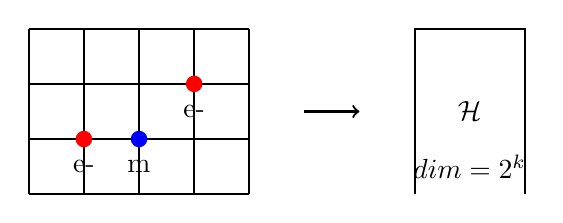
\begin{tikzpicture}[scale=0.7]
% Surface with defects
\draw[thick] (0,0) grid (4,3);
\fill[red] (1,1) circle (0.15);
\fill[red] (3,2) circle (0.15);
\fill[blue] (2,1) circle (0.15);
\node at (1,0.5) {e-};
\node at (3,1.5) {e-};
\node at (2,0.5) {m};

% Arrow
\draw[thick,->] (5,1.5) -- (6,1.5);

% Hilbert space
\draw[thick] (7,0) -- (7,3) -- (9,3) -- (9,0);
\node at (8,1.5) {$\mathcal{H}$};
\node at (8,0.5) {$\text{dim}=2^k$};
\end{tikzpicture}
\end{center}

\subsection{Functorial Field Theory}

\subsubsection{TQFT Axioms Diagrammatically}

The functorial nature of TQFT:

\[
\begin{tikzcd}[row sep=small]
\text{Cob}_n \arrow[rr, "Z"] & & \text{Vect} \\
M_1 \sqcup M_2 \arrow[dd, "\Sigma"] \arrow[rr, mapsto] & & 
Z(M_1) \otimes Z(M_2) \arrow[dd, "Z(\Sigma)"] \\
& & \\
M' \arrow[rr, mapsto] & & Z(M')
\end{tikzcd}
\]

\subsubsection{Chern-Simons Theory}

The Chern-Simons TQFT assigns:
\begin{align}
Z(S^1) &= \mathbb{C}[G] \quad \text{(Group algebra)} \\
Z(T^2) &= \text{Rep}(G) \quad \text{(Representation ring)} \\
Z(S^3) &= \mathbb{C} \quad \text{(Complex numbers)}
\end{align}

With the crucial three-manifold invariant:
\[
Z(M^3) = \int_{\mathcal{A}/\mathcal{G}} \mathcal{D}A \, e^{ik\,\text{CS}(A)}
\]

\subsection{Gauge Theory Categorically}

\subsubsection{Principal Bundles as Functors}

Gauge fields as natural transformations:

\[
\begin{tikzcd}[row sep=large, column sep=large]
\text{Open}(M) \arrow[r, "P", bend left=20] \arrow[r, "P'", bend right=20] & 
\text{BG} \\
\end{tikzcd}
\]

With gauge transformation $g: P \Rightarrow P'$ satisfying:
\[
\begin{tikzcd}
P(U \cap V) \arrow[r, "g_{U \cap V}"] \arrow[d, "\text{res}"'] & 
P'(U \cap V) \arrow[d, "\text{res}"] \\
P(U) \times P(V) \arrow[r, "g_U \times g_V"'] & 
P'(U) \times P'(V)
\end{tikzcd}
\]

\subsubsection{Yang-Mills as Variational Functor}

The Yang-Mills functional as a natural transformation:

\[
\text{YM}: \text{Conn} \Rightarrow \mathbb{R}_{\geq 0}
\]

With critical points (instantons) characterized by:
\[
\begin{tikzcd}
\text{Conn} \arrow[r, "\text{YM}"] \arrow[d, "F"'] & 
\mathbb{R}_{\geq 0} \\
\Omega^2(M, \mathfrak{g}) \arrow[ur, "\|F\|^2"'] &
\end{tikzcd}
\]

\subsection{Quantum Information Diagrams}

\subsubsection{Teleportation Protocol}

Quantum teleportation as functorial composition:

\[
\begin{tikzcd}[column sep=small, row sep=large]
\vert\psi\rangle \otimes \vert\Phi^+\rangle \arrow[r, "\text{Bell}"] & 
\text{Entangled}_3 \arrow[r, "\text{Measure}_{12}"] & 
\vert 00\rangle + \vert 11\rangle \arrow[d, "\text{Classical}"] \\
& & 
\text{Bits} \arrow[d, "\text{Unitary}"] \\
\vert\psi\rangle \arrow[uurr, phantom, "\text{Teleport}"] & & 
\vert\psi\rangle
\end{tikzcd}
\]

\subsubsection{Quantum Computation as Braiding}

Topological quantum computation via anyons:

\begin{center}
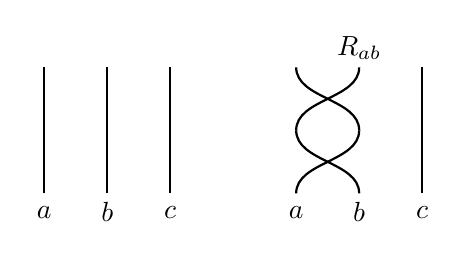
\begin{tikzpicture}[scale=0.8]
% Initial anyons
\draw[thick] (0,0) -- (0,2);
\draw[thick] (1,0) -- (1,2);
\draw[thick] (2,0) -- (2,2);
\node at (0,-0.3) {$a$};
\node at (1,-0.3) {$b$};
\node at (2,-0.3) {$c$};

% Braiding
\draw[thick] (4,0) .. controls (4,0.5) and (5,0.5) .. (5,1);
\draw[thick] (5,1) .. controls (5,1.5) and (4,1.5) .. (4,2);
\draw[thick] (5,0) .. controls (5,0.5) and (4,0.5) .. (4,1);
\draw[thick] (4,1) .. controls (4,1.5) and (5,1.5) .. (5,2);
\draw[thick] (6,0) -- (6,2);

% Result
\node at (4,-0.3) {$a$};
\node at (5,-0.3) {$b$};
\node at (6,-0.3) {$c$};
\node at (5,2.3) {$R_{ab}$};
\end{tikzpicture}
\end{center}

\subsection{Emergence and Limits}

\subsubsection{Classical Limit Functor}

The emergence of classical mechanics:

\[
\begin{tikzcd}[row sep=large, column sep=large]
\text{Hilb} \arrow[r, "\hbar \to 0"] \arrow[d, "\rho"'] & 
\text{Phase} \arrow[d, "\mu"] \\
\text{States} \arrow[r, "\text{Wigner}"'] & 
\text{Measures}
\end{tikzcd}
\]

Where the Wigner function provides the bridge:
\[
W_\rho(q,p) = \frac{1}{(2\pi\hbar)^n} \int \psi^*(q+\tfrac{x}{2}) \psi(q-\tfrac{x}{2}) e^{ipx/\hbar} dx
\]

\subsubsection{Thermodynamic Limit}

Statistical mechanics emerging via limits:

\[
\begin{tikzcd}
\text{Micro}_N \arrow[r, "N \to \infty"] \arrow[d, "\text{partition}"'] & 
\text{Thermo} \arrow[d, "S"] \\
\mathbb{C}^{2^N} \arrow[r, "\text{trace}"'] & 
\mathbb{R}
\end{tikzcd}
\]

\subsection{Concrete Calculations}

\subsubsection{Categorical Quantum Mechanics Example}

Computing with spider diagrams for GHZ state preparation:

\begin{center}
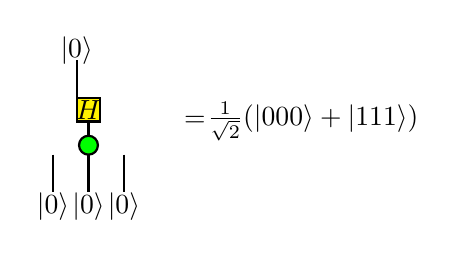
\begin{tikzpicture}[scale=0.6]
% Input
\node at (0,3) {$|0\rangle$};
\draw[thick] (0,2.8) -- (0,2);

% Hadamard
\draw[thick,fill=yellow] (0,2) rectangle (0.5,1.5);
\node at (0.25,1.75) {$H$};

% Spider
\draw[thick] (0.25,1.5) -- (0.25,1);
\draw[thick,fill=green] (0.25,1) circle (0.2);
\draw[thick] (-0.5,0.8) -- (-0.5,0);
\draw[thick] (0.25,0.8) -- (0.25,0);
\draw[thick] (1,0.8) -- (1,0);

% Outputs
\node at (-0.5,-0.3) {$|0\rangle$};
\node at (0.25,-0.3) {$|0\rangle$};
\node at (1,-0.3) {$|0\rangle$};

% Equals
\node at (2.5,1.5) {$=$};

% Result
\node at (5,1.5) {$\frac{1}{\sqrt{2}}(|000\rangle + |111\rangle)$};
\end{tikzpicture}
\end{center}

\subsubsection{Functorial Dynamics}

Time evolution as a functor-preserving structure:

\[
\begin{tikzcd}[row sep=large]
\text{Obs} \times \mathbb{R} \arrow[r, "U_t"] \arrow[d, "\{-,-\}"'] & 
\text{Obs} \arrow[d, "[-,-]"] \\
\text{Poisson} \arrow[r, "e^{t\{H,-\}}"'] & 
\text{Lie}
\end{tikzcd}
\]

\subsection{Advanced Constructions}

\subsubsection{Higher Gauge Theory}

2-gauge theory with gerbes:

\[
\begin{tikzcd}
C^1(M,G) \arrow[r, "\delta"] \arrow[d, "B"'] & 
C^2(M,G) \arrow[d, "B"] \\
\Omega^1(M,\mathfrak{g}) \arrow[r, "d"'] & 
\Omega^2(M,\mathfrak{g})
\end{tikzcd}
\]

\subsubsection{Quantum Gravity Emergence}

Spacetime from entanglement:

\[
\begin{tikzcd}
\text{CFT}_{\text{boundary}} \arrow[r, "\text{AdS/CFT}"] \arrow[d, "\text{entangle}"'] & 
\text{Gravity}_{\text{bulk}} \arrow[d, "\text{geometry}"] \\
\text{TensorNetwork} \arrow[r, "\text{emerge}"'] & 
\text{Spacetime}
\end{tikzcd}
\]

\subsection{Computational Implementation}

\subsubsection{Verified Quantum Algorithms}

Grover's algorithm with categorical proof:

\begin{verbatim}
-- Grover operator as natural transformation
grover :: Nat (State n) (State n)
grover = inversion . oracle
  where
    oracle = markTarget
    inversion = 2 |> uniformSuperposition >< uniformSuperposition <| - id

-- Categorical proof of quadratic speedup
speedupProof :: Proof (Iterations grover == O(sqrt n))
speedupProof = categoricalInduction {
  base = trivial,
  step = preservesSuperposition <> amplitudeAnalysis
}
\end{verbatim}

\subsubsection{Diagrammatic Reasoning Engine}

Automated diagram manipulation:

\begin{verbatim}
-- Spider fusion rule
spiderFusion :: Diagram -> Diagram
spiderFusion (Spider n `compose` Spider m) = Spider (n + m)

-- Bialgebra law
bialgebraLaw :: Proof (delta . nabla == (nabla `tensor` nabla) . (id `tensor` sigma `tensor` id) . (delta `tensor` delta))

-- Automated simplification
simplify :: Diagram -> Diagram
simplify = fixpoint (spiderFusion <> copyRule <> bialgebraLaw)
\end{verbatim}

\subsection{Summary of Key Diagrams}

The diagrams presented illustrate:

\begin{enumerate}[leftmargin=*]
\item \textbf{Functorial Structure}: Physical theories as functors between categories
\item \textbf{Compositional Nature}: Complex phenomena built from simple categorical pieces
\item \textbf{Universal Properties}: Physical laws as universal constructions
\item \textbf{Computational Content}: Every diagram translates to executable code
\end{enumerate}

These concrete examples demonstrate that functorial physics is not merely abstract formalism but provides practical tools for understanding and computing physical phenomena. The convergence of mathematical elegance, physical insight, and computational tractability suggests we have found the natural language of physics.